\documentclass[A4paper,11pt]{article}
\usepackage{amsmath,amssymb,amsfonts,amsthm}
\usepackage{enumerate}
%\usepackage{enumitem}
\usepackage{paralist}
\usepackage{graphics} %% add this and next lines if pictures should be in esp format
\usepackage{float}
\usepackage{epsfig} %For pictures: screened artwork should be set up with an 85 or 100 line screen
\usepackage{graphicx}
\usepackage{epstopdf}%This is to transfer .eps figure to .pdf figure; please compile your paper using PDFLeTex or PDFTeXify.
\usepackage[colorlinks=true]{hyperref}
\hypersetup{urlcolor=blue, citecolor=red}
%\usepackage{hyperref}

\usepackage{bm}
\usepackage{color}

%  \textheight=8.2 true in
%   \textwidth=5.0 true in
%    \topmargin 30pt
%     \setcounter{page}{1}

\usepackage[a4paper]{geometry}

\newtheorem{theorem}{Theorem}[section]
\newtheorem{corollary}{Corollary}
\newtheorem*{main}{Main Theorem}
\newtheorem{lemma}[theorem]{Lemma}
\newtheorem{proposition}{Proposition}
\newtheorem{conjecture}{Conjecture}
\newtheorem*{problem}{Problem}
\theoremstyle{definition}
\newtheorem{definition}[theorem]{Definition}
\newtheorem{remark}{Remark}
\newtheorem{example}{Example}
\newtheorem*{notation}{Notation}
\newcommand{\ep}{\varepsilon}
\newcommand{\eps}[1]{{#1}_{\varepsilon}}

\newcommand{\vnorm}[1]{\left\| #1 \right\|}
\newcommand{\scalarp}[1]{\left\langle #1 \right\rangle}
\newcommand{\redd}[1]{{\color{red}{#1}}}

\newcommand{\R}{\mathbb{R}}
\DeclareMathOperator{\supp}{supp}
\DeclareMathOperator{\sgn}{sgn}
\DeclareMathOperator{\diag}{diag}


\title{Interaction Kernel Learning in Multi-Agent Dynamical System}

\author{M. Bongini, M. Fornasier, M. Hansen, M. Maggioni}


\begin{document}
\maketitle

\bigskip


%The abstract of your paper
\begin{abstract}
We address the problem of...
\end{abstract}

\section{The framework}

We assume that we are given $N$ agents whose dynamics satisfies, for every $t > 0$, the following set of ordinary differential equations
\begin{align*}
\begin{cases}
\dot{x_i}(t) = v_i(t), \\
\dot{v_i}(t) = \frac{1}{N}\sum^N_{j = 1} a(\vnorm{x_j(t) - x_i(t)}_{\ell^d_2})(v_j(t) - v_i(t)),
\end{cases}
\end{align*}
where the \emph{state parameter} $x_i$ and the \emph{consensus parameter} $v_i$ of the $i$-th agent both lie in the euclidean space $\mathbb{R}^d$ equipped with the euclidean norm $\vnorm{\cdot}_{\ell^d_2}$ (whose subscript shall be omitted when clear from the context).

The \emph{interaction kernel} $a$ is assumed to be unknown.

\section{Numerical experiments}

\subsection{The algorithm}

The algorithm takes as inputs a snapshots' dataset $\mathcal{D} = \{(x_i(n \Delta t), v_i(n \Delta t)) \mid i = 1, \ldots, N, n = 0, \ldots [T/\Delta t]\}$ in which each couple $(x_i(n \Delta t), v_i(n \Delta t))$ represents the position and the velocity of the $i$-th agent at time $n \Delta t$. From this dataset we can calculate the empirical accelerations of the agents at time $n \Delta t$ as
\begin{align*}
v^{\prime}_i(n \Delta t) := \frac{v_i((n+1)\Delta t) - v_i(n \Delta t)}{\Delta t}.
\end{align*}
To determine the function $a$, we consider, for any $n = 0, \ldots [T/\Delta t]$, the function
\begin{align*}
\psi^{\mathcal{D}}_n(a) := \frac{1}{N} \sum^N_{i = 1} a\left(\vnorm{x_i(n \Delta t) - x_j(n \Delta t)}\right)(v_j(n \Delta t) - v_i(n \Delta t)) - v^{\prime}_i(n \Delta t),
\end{align*}
and consider $\psi^{\mathcal{D}}(a) = \left[\psi^{\mathcal{D}}_0(a), \ldots, \psi^{\mathcal{D}}_{[T/\Delta t]}(a)\right]$.

The idea is to minimize the quantity $\vnorm{\psi^{\mathcal{D}}(f)}^2$ in a set of functions $\Lambda_m$ in which a suitable approximation of the unknown function $a$ lives: we start from a function space $\Lambda_0$ and enlarge it at every step $m$ until we reach the desired accuracy for $a$. 

To this end, given a vector $\mathbf{t}^m = (t^m_1, \ldots, t^m_{k_m}) \in \mathbb{R}^{k_m}$ of nodes in increasing order, we take $\Lambda_m$ to be the linear subspace of dimension $k_m - d$ generated by the spline basis of order $d$ with nodal basis $\mathbf{t}^m$, that is
\begin{align*}
\Lambda_m = \textup{span}\left(\{\varphi^{\mathbf{t}^m}_{\ell}\}_{\ell = 1}^{k_{m}-d}\right).
\end{align*}
Hence, we assume that a good approximation of the function $a$ lies in $\Lambda_m$, that is it has the form
\begin{align*}
a \approx \sum^{k_{m}-d}_{\ell = 1} c_{\ell} \varphi^{\mathbf{t}^m}_{\ell},
\end{align*}
for given $\mathbf{c} = (c_1, \ldots, c_{k_m - d}) \in \mathbb{R}^{k_m - d}$. This ansatz allow us to rewrite $\psi^{\mathcal{D}}$ as
\begin{eqnarray*}
\psi^{\mathcal{D}}_n(a) \approx \psi^{\mathcal{D}, \mathbf{t}^m}_n(\mathbf{c}) & = & \frac{1}{N} \sum^N_{j = 1} \sum^{k_{n}-d}_{\ell = 1} c_{\ell} \varphi^{\mathbf{t}^m}_{\ell} \!\! \left(\vnorm{x_i(n \Delta t) - x_j(n \Delta t)}\right)(v_j(n \Delta t) - v_i(n \Delta t)) \\
& & - v^{\prime}_i(n \Delta t) \\
& = & \mathbf{c} \cdot A^{\mathbf{t}^m}_n - \mathbf{d}_n,
\end{eqnarray*}
where, for every $n = 0, \ldots, [T/\Delta t]$, we set $(\mathbf{d}_n)_i = v^{\prime}_i(n \Delta t)$ and
\begin{align*}
(A_n^{\mathbf{t}^m})_{\ell i} = \frac{1}{N} \sum^N_{j = 1}\varphi^{\mathbf{t}^m}_{\ell} \left(\vnorm{x_i(n \Delta t) - x_j(n \Delta t)}\right)(v_j(n \Delta t) - v_i(n \Delta t)).
\end{align*}
This means that, for every $m$,
\begin{eqnarray*}
\psi^{\mathcal{D}, \mathbf{t}^m}(\mathbf{c}) = \mathbf{c} \cdot A^{\mathbf{t}^m} - \mathbf{d}, & \text{ where } & A^{\mathbf{t}^m} = [A^{\mathbf{t}^m}_0, \ldots, A^{\mathbf{t}^m}_{[T/\Delta t]}] \text{ and } \mathbf{d} = [\mathbf{d}_0, \ldots, \mathbf{d}_{[T/\Delta t]}].
\end{eqnarray*}
To clarify the situation, we point out that $A_n^{\mathbf{t}^m} \in \mathbb{R}^{(k_m - d)\times N}$ and $\mathbf{d}_n  \in \mathbb{R}^N$, thus $A^{\mathbf{t}^m} \in \mathbb{R}^{(k_m - d) \times N \times [T/\Delta t]}$ and $\mathbf{d} \in \mathbb{R}^{N \times [T/\Delta t]}$.

This means that, for every $m$, we are facing the following least-squares minimization procedure:
\begin{align*}
P(m) := \text{minimize } \vnorm{\mathbf{c} \cdot A^{\mathbf{t}^m} - \mathbf{d}}^2 \text{ among all } \mathbf{c} \in \mathbb{R}^{k_m - d}.
\end{align*}

\subsubsection{Refinement procedure}

As $\mathbf{t}^0$ we take the vector $\left(j \frac{M}{s}\right)_{j = 1}^{s}$ for given $M > 0$ and $s > 1$ ($s$ is an integer), while as $\mathbf{t}^1$ we take $\left(j \frac{M}{2s}\right)_{j = 1}^{2s}$ for the same $M$ and $s$ as before. We then solve the two minimization problems $P(0)$ and $P(1)$ (whose solutions we indicate with $\mathbf{c}^0$ and $\mathbf{c}^1$, respectively) and consider the two obtained approximations of the interaction kernel, namely:
\begin{eqnarray*}
a_0 = \sum^{s - d}_{\ell} c^0_{\ell} \varphi^{\mathbf{t}^0}_{\ell} & \text{and} & a_1 = \sum^{2s - d}_{\ell} c^1_{\ell} \varphi^{\mathbf{t}^1}_{\ell},
\end{eqnarray*}
where we remark that $d$ is the order of the spline basis elements.

At this point, we compute the forward difference quotients of $a_0$ and $a_1$ at every point of $\mathbf{t}^1$, that is for every $j$ such that $t^1_{j+1} \in \mathbf{t}^1$ we compute
\begin{align*}
a^{\prime}_i(t^1_j;t^1_{j+1}) = \frac{a_i(t^1_{j+1}) - a_i(t^1_j)}{t^1_{j+1} - t^1_j} \quad \text{ for } \quad i = 1,2.
\end{align*}
We set a tolerance $\varepsilon > 0$ and we indicate with
\begin{align*}
I^1_{\varepsilon} = \left\{ (t^1_j, t^1_{j+1}) \in \mathbb{R}^2 \mid \vnorm{a^{\prime}_1(t^1_j;t^1_{j+1}) - a^{\prime}_0(t^1_j;t^1_{j+1})} > \varepsilon \right\}
\end{align*}
the set of couples of nodes for which the forward differences differ more than the tolerance. Hence, we construct the next nodal set $\mathbf{t}^2$ by taking all the node in $\mathbf{t}^1$, adding the middle point of every couple in the set $I^1_{\varepsilon}$ and then reordering in increasing order: this means that, $t \in \mathbf{t}^2$ if and only if $t \in \mathbf{t}^1$ or there exist a couple $(t^1_j, t^1_{j+1}) \in I^1_{\varepsilon}$ such that
\begin{align*}
t = \frac{t^1_{j+1} + t^1_j}{2}.
\end{align*}
At this point we repeat the construction of $I^2_{\varepsilon}$ and $\mathbf{t}^3$ as before, until we have $I^m_{\varepsilon} = \emptyset$ for some $m$.

\subsubsection{Known issues}

The algorithm has basically two issues.
\begin{itemize}
\item the oscillatory effect at $0$: this is due to the fact that the elements of the spline basis are zero at their starting node. This problem seems to be not solvable with the trick of taking as first node in $\mathbf{t}^0$ the point $-1$. It could be solved by imposing that the new refinement does not introduce a ``worse'' oscillatory effect than the old one. How much oscillatory an approximation is can be measured by taking the sum of the moduli of the finite differences of the approximation: the higher this value is, the more oscillatory the approximation is.
\item the introduction of new points worsen previously accurate part of the approximation: this seems to occur often. I don't know if this issue is related to the first one.
\end{itemize}

\subsection{Smooth kernel}

For the first test, we consider the following interaction kernel:
\begin{align*}
a(r) = \frac{100}{(100+r^2)^2} + \frac{0.04}{30 + (r - 20)^2} - \frac{0.04}{(30 + (r - 40)^2}.
\end{align*}
portrayed in red in Figure \ref{fig:7}.

\begin{figure}[H]
\centering
\begin{minipage}{.33\textwidth}
  \centering
  \vspace{0.22cm}
  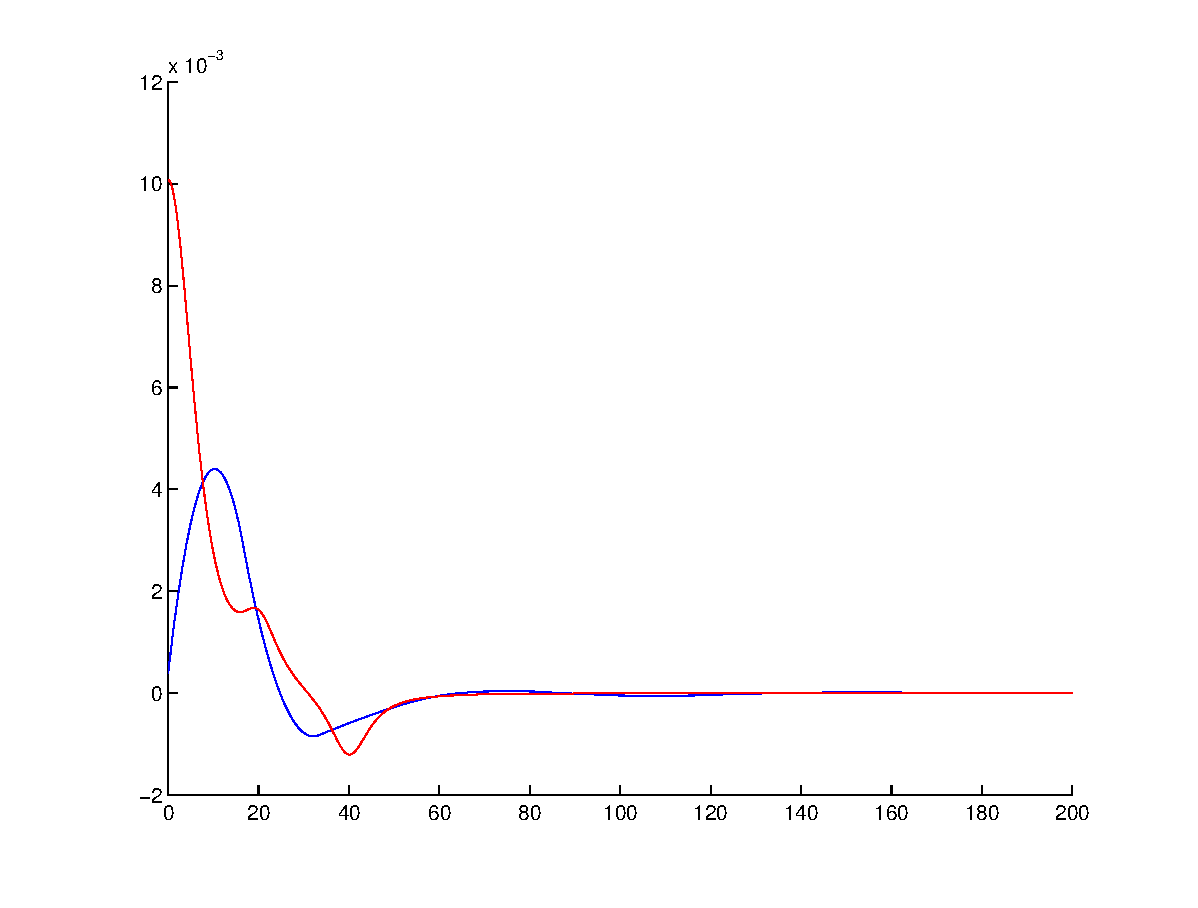
\includegraphics[scale=0.25]{pictures/Example7/Fig2.eps}
  \label{fig:7_2}
\end{minipage}%
\begin{minipage}{.33\textwidth}
  \centering
  \vspace{0.2cm}
  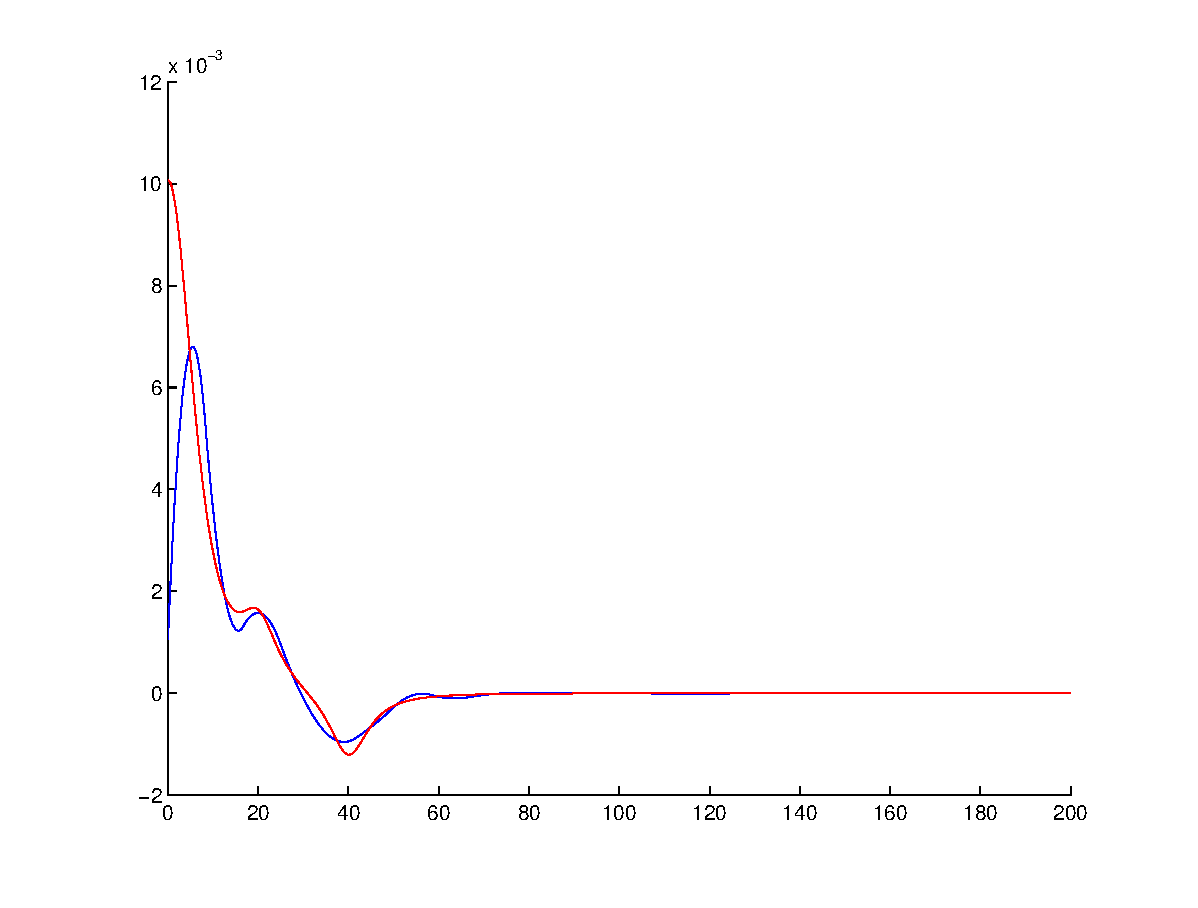
\includegraphics[scale=0.25]{pictures/Example7/Fig3.eps}
  \label{fig:7_3}
\end{minipage}%
\begin{minipage}{.33\textwidth}
  \centering
  \vspace{0.2cm}
  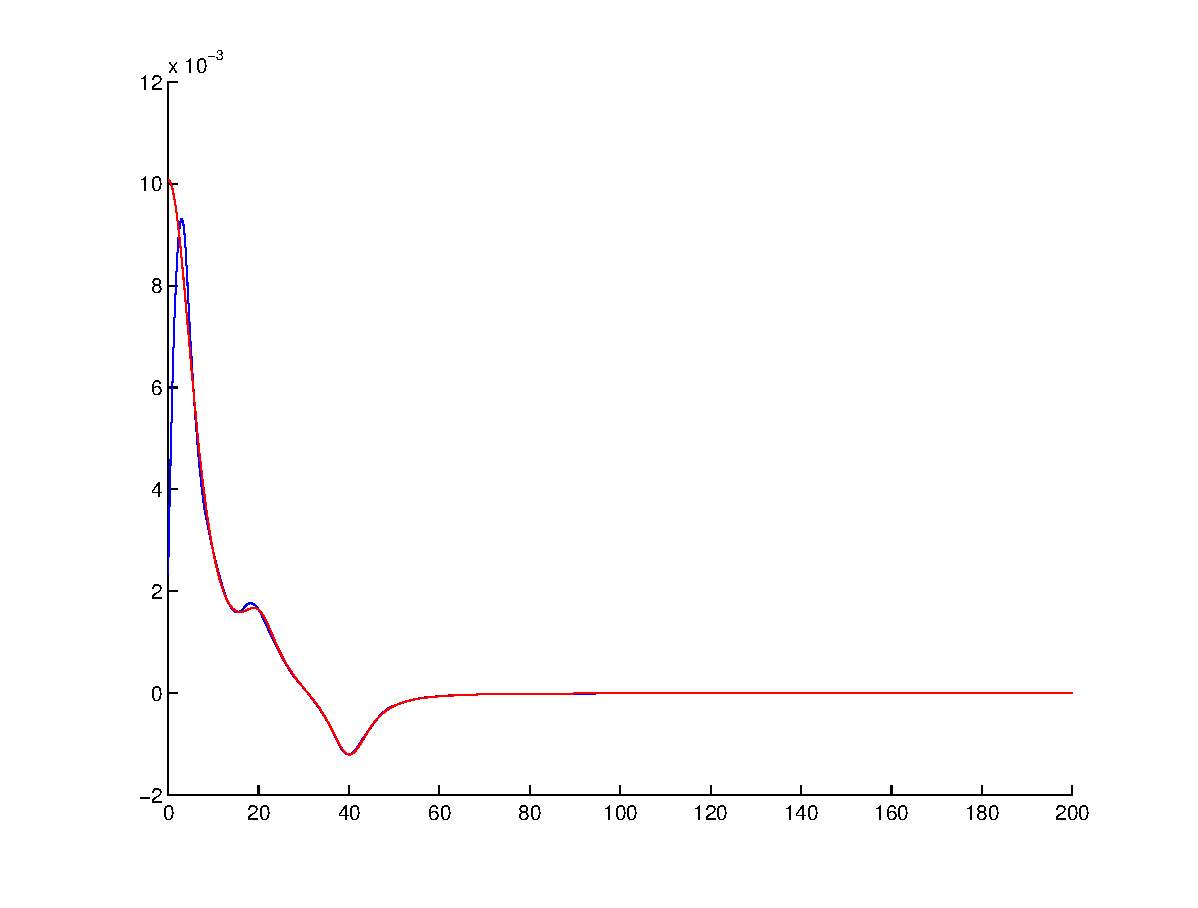
\includegraphics[scale=0.25]{pictures/Example7/Fig4.eps}
  \label{fig:7_4}
\end{minipage}%
\end{figure}

\begin{figure}[H]
\centering
\begin{minipage}{.33\textwidth}
  \centering
  \vspace{0.22cm}
  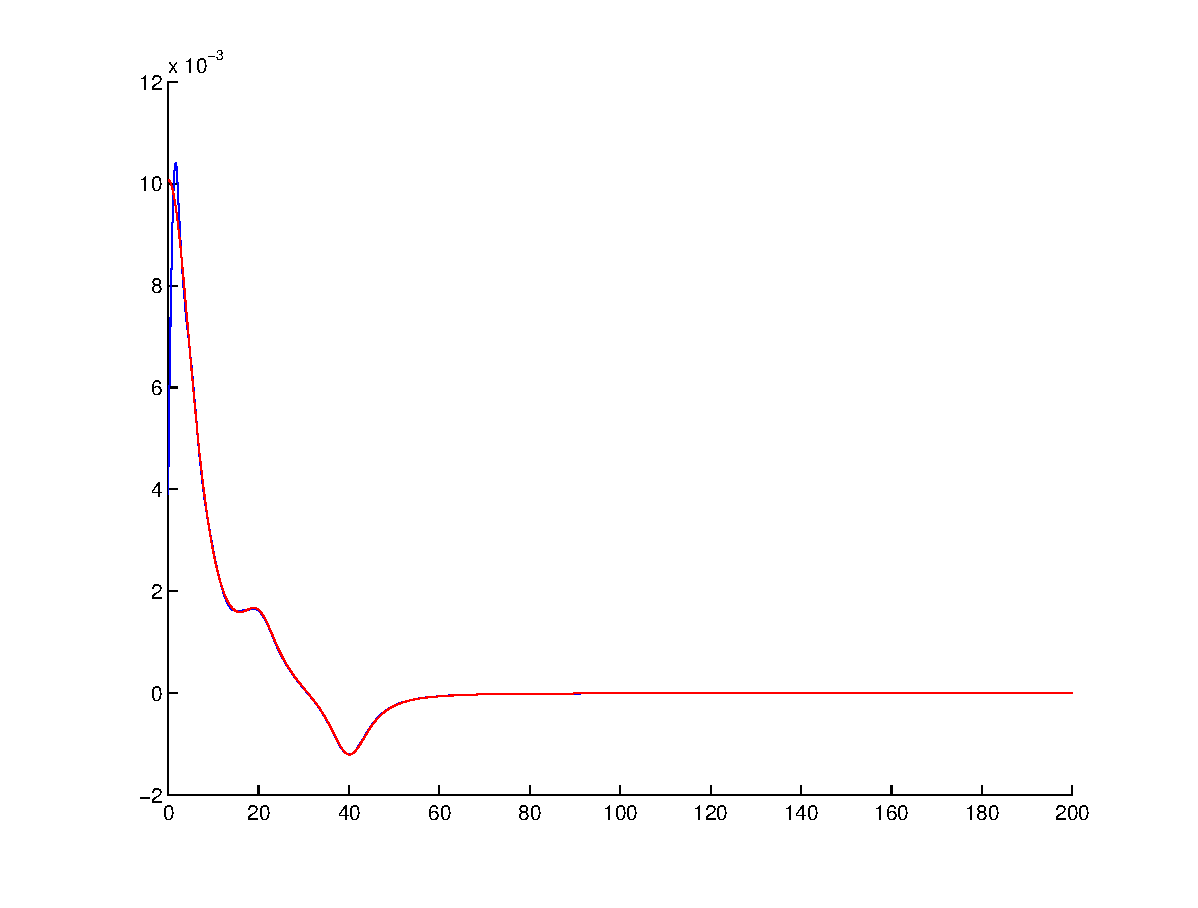
\includegraphics[scale=0.25]{pictures/Example7/Fig5.eps}
  \label{fig:7_5}
\end{minipage}%
\begin{minipage}{.33\textwidth}
  \centering
  \vspace{0.2cm}
  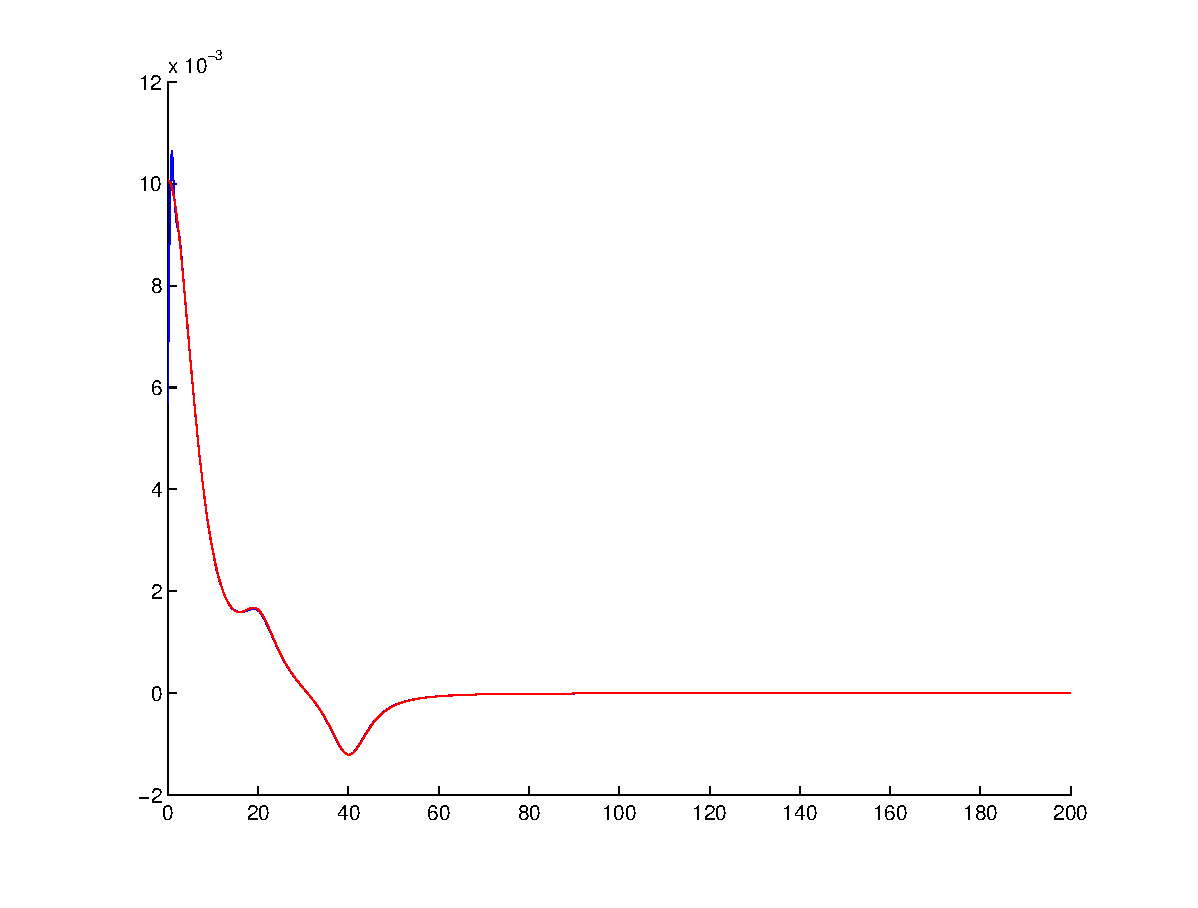
\includegraphics[scale=0.25]{pictures/Example7/Fig6.eps}
  \label{fig:7_6}
\end{minipage}%
\begin{minipage}{.33\textwidth}
  \centering
  \vspace{0.2cm}
  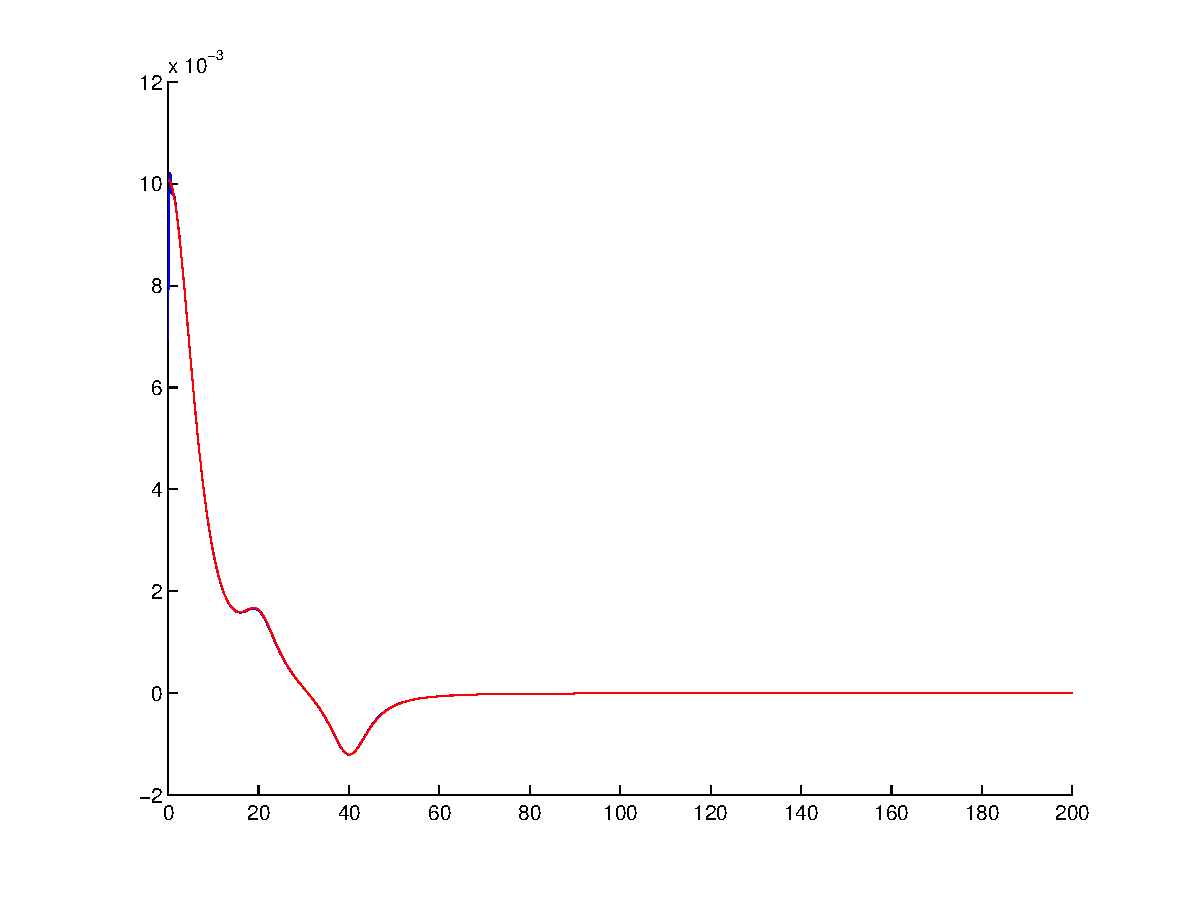
\includegraphics[scale=0.25]{pictures/Example7/Fig7.eps}
  \label{fig:7_7}
\end{minipage}%
\caption{}
\label{fig:7}
\end{figure}

\subsection{Oscillatory kernel}

For the second test, we take the following highly oscillating interaction kernel:
\begin{align*}
a(r) = \sin(3r) \frac{100}{(100+r^2)^{\frac{4}{5}}} + \sin\left(\frac{r}{10}\right) \frac{100}{30 + (r - 50)^2},
\end{align*}
depicted in red in Figure \ref{fig:8}.

\begin{figure}[H]
\centering
\begin{minipage}{.33\textwidth}
  \centering
  \vspace{0.22cm}
  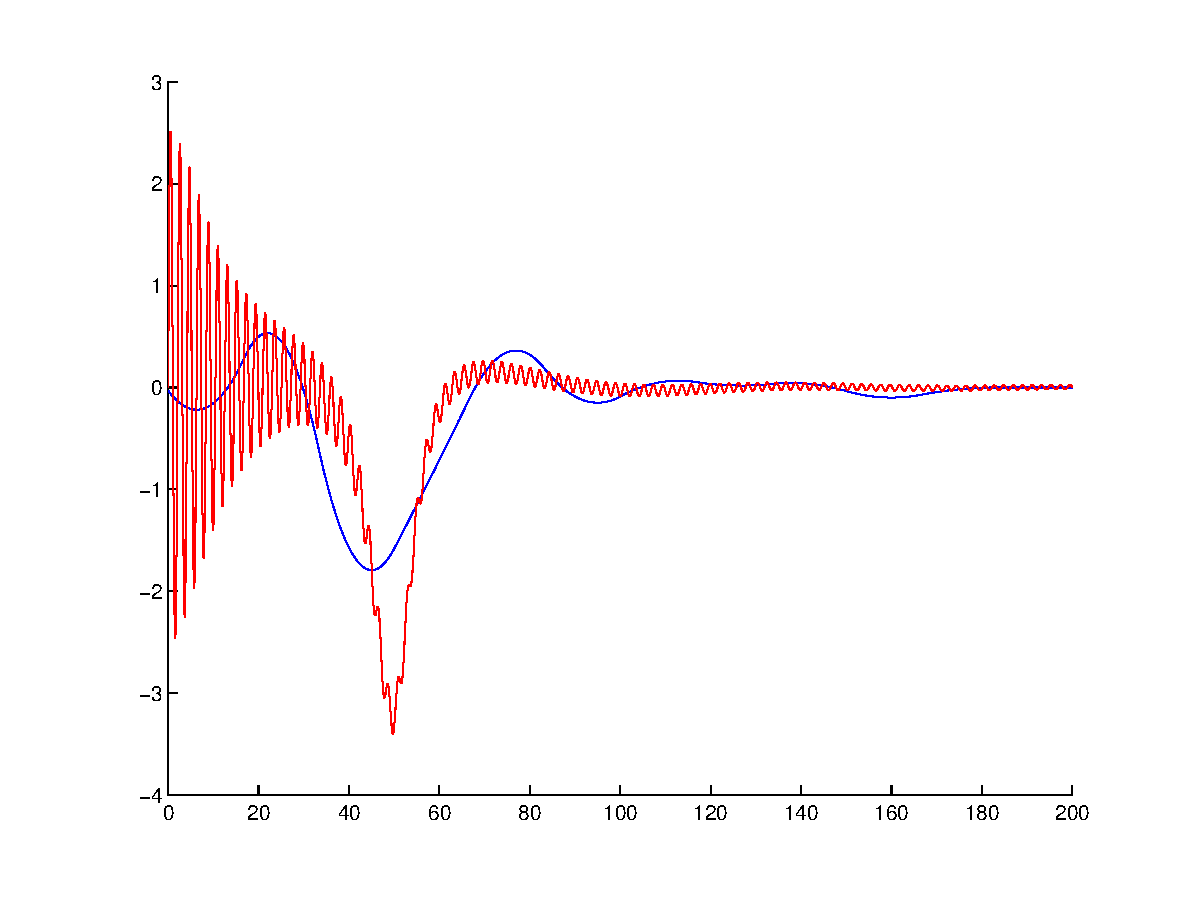
\includegraphics[scale=0.25]{pictures/Example8/Fig2.eps}
  \label{fig:8_2}
\end{minipage}%
\begin{minipage}{.33\textwidth}
  \centering
  \vspace{0.2cm}
  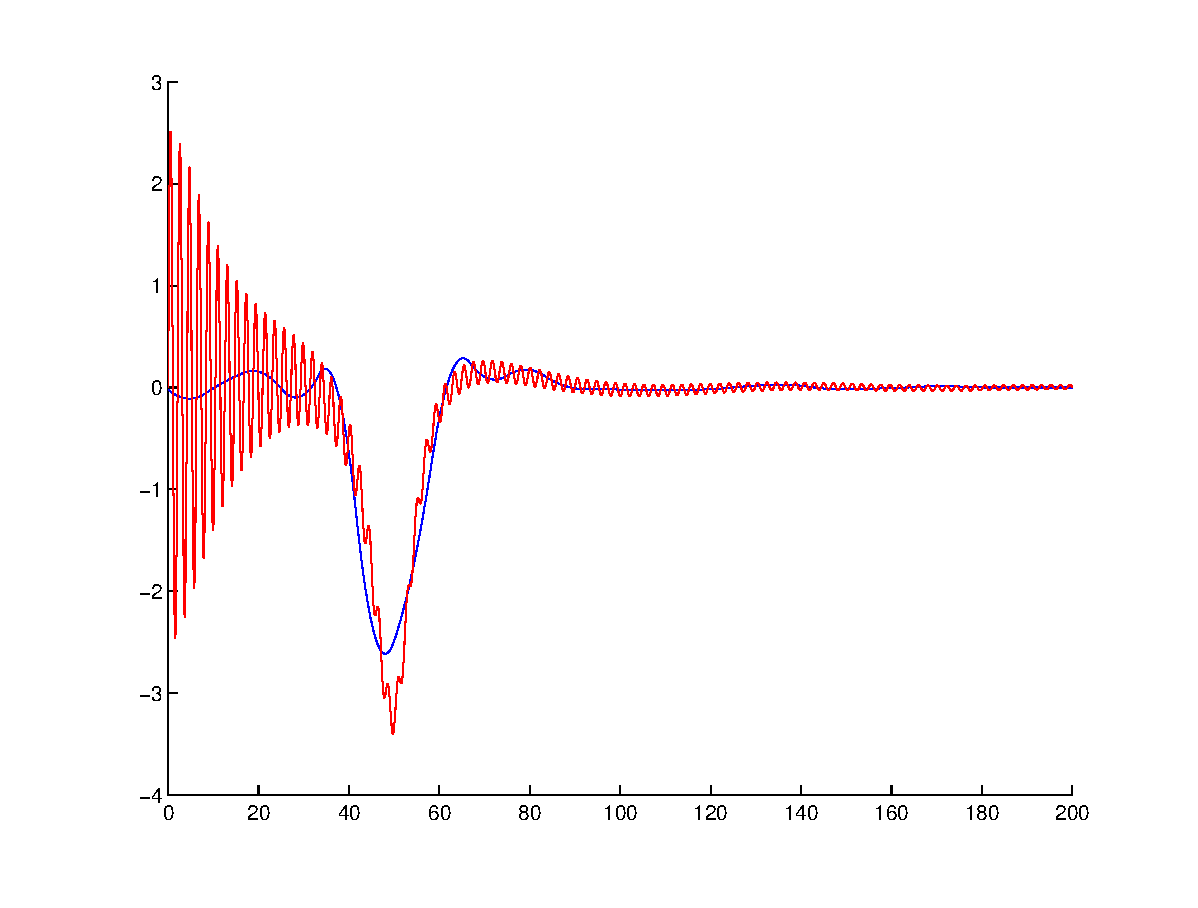
\includegraphics[scale=0.25]{pictures/Example8/Fig3.eps}
  \label{fig:8_3}
\end{minipage}%
\begin{minipage}{.33\textwidth}
  \centering
  \vspace{0.2cm}
  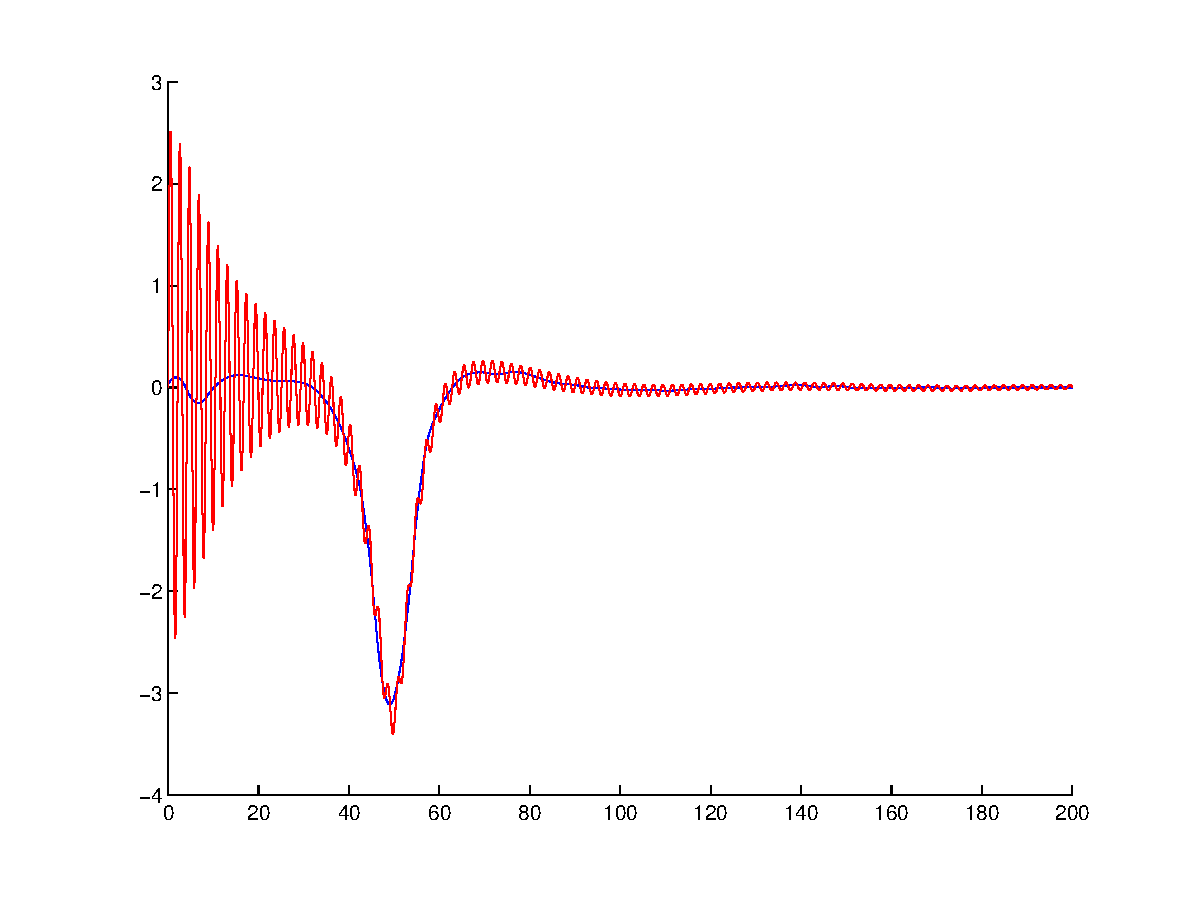
\includegraphics[scale=0.25]{pictures/Example8/Fig4.eps}
  \label{fig:8_4}
\end{minipage}%
\end{figure}

\begin{figure}[H]
\centering
\begin{minipage}{.33\textwidth}
  \centering
  \vspace{0.22cm}
  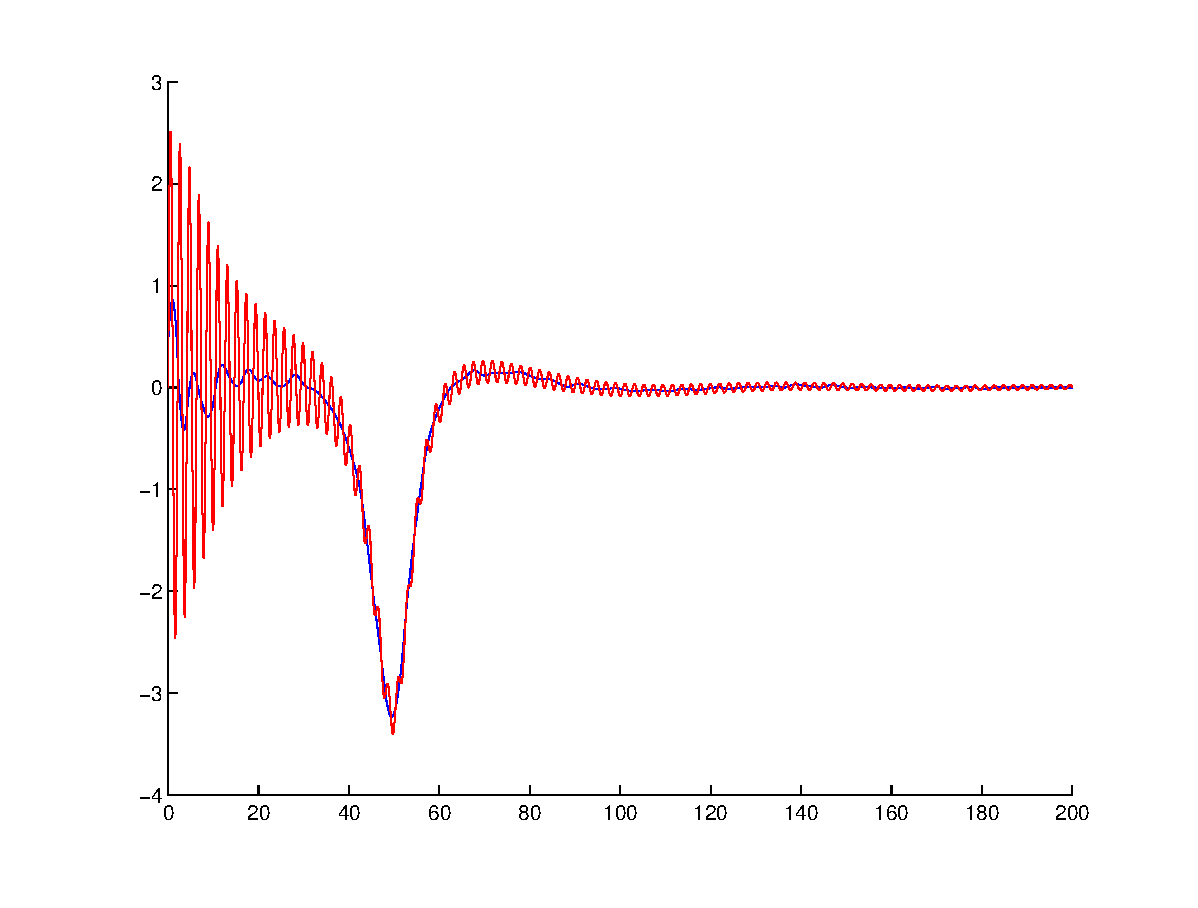
\includegraphics[scale=0.25]{pictures/Example8/Fig5.eps}
  \label{fig:8_5}
\end{minipage}%
\begin{minipage}{.33\textwidth}
  \centering
  \vspace{0.2cm}
  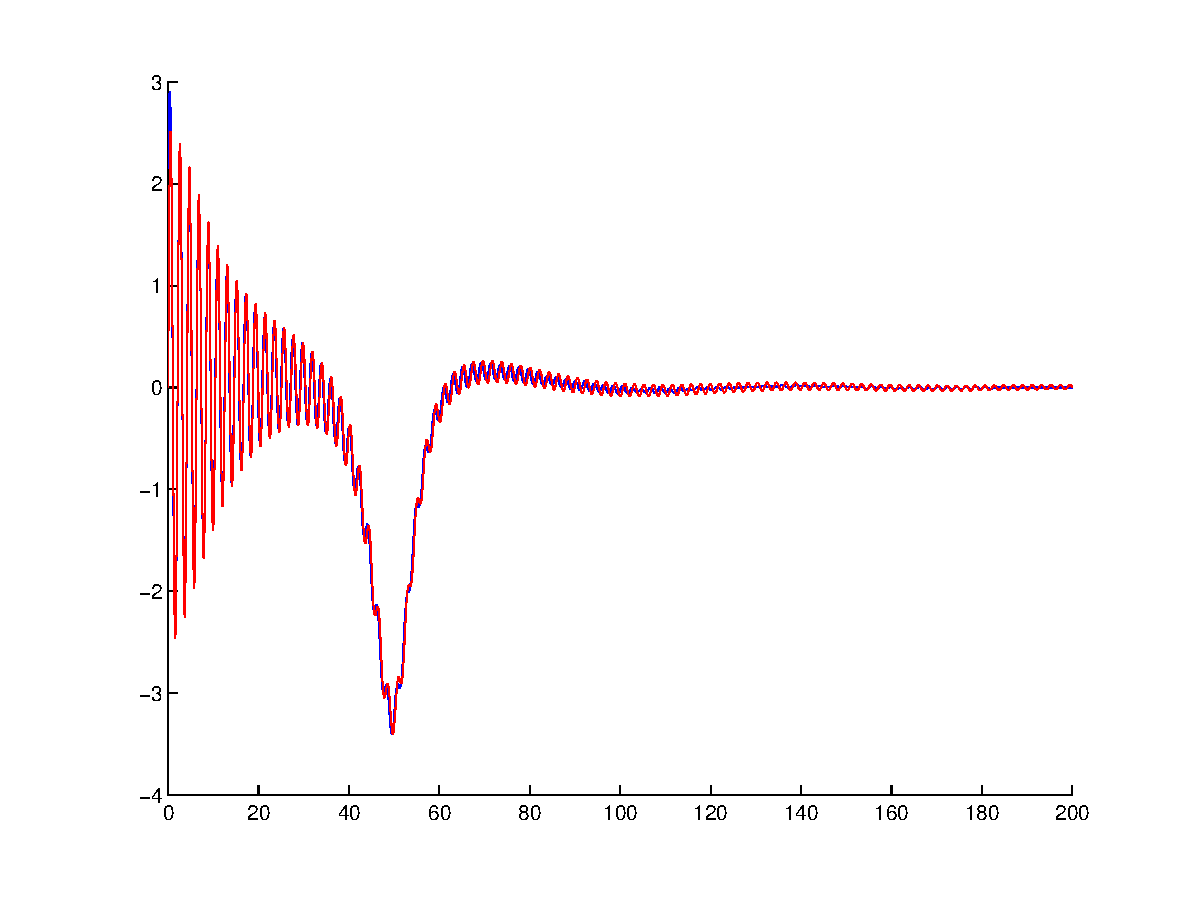
\includegraphics[scale=0.25]{pictures/Example8/Fig6.eps}
  \label{fig:8_6}
\end{minipage}%
\begin{minipage}{.33\textwidth}
  \centering
  \vspace{0.2cm}
  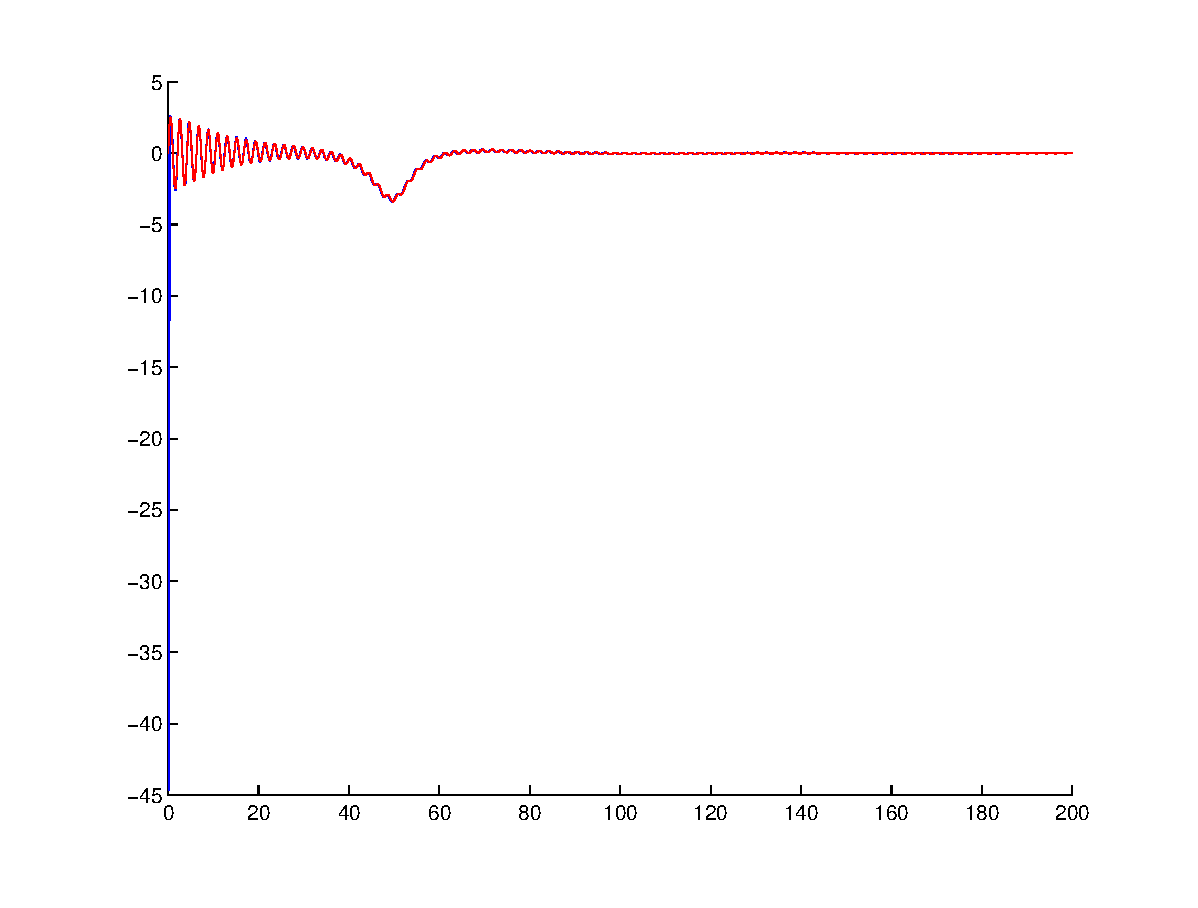
\includegraphics[scale=0.25]{pictures/Example8/Fig9.eps}
  \label{fig:8_7}
\end{minipage}%
\caption{}
\label{fig:8}
\end{figure}

The difficulty in correctly approximating the value of the interaction kernel at 0 can be seen in the bottom-left picture. The oscillatory effect that takes place adds up at every iteration of the algorithm and has a malicious effect on the whole approximation.

\subsection{Discontinuous kernel}

As a last example, we consider a discontinuous interaction kernel of the form
\begin{align*}
a(r) = H(10 - r)\frac{2}{(100+r^2)^{\frac{4}{5}}} + H(r - 20)H(40 - r)\frac{2}{35 + (r - 40)^2} + H(r - 45)\frac{2}{35 + (r - 40)^2},
\end{align*}
where $H$ is the Heaviside function. It is again portrayed in red in Figure \ref{fig:9}. The arising of a Gibbs phenomenon at the discontinuity jumps of the interaction kernel is clearly visible.

\begin{figure}[H]
\centering
\begin{minipage}{.33\textwidth}
  \centering
  \vspace{0.22cm}
  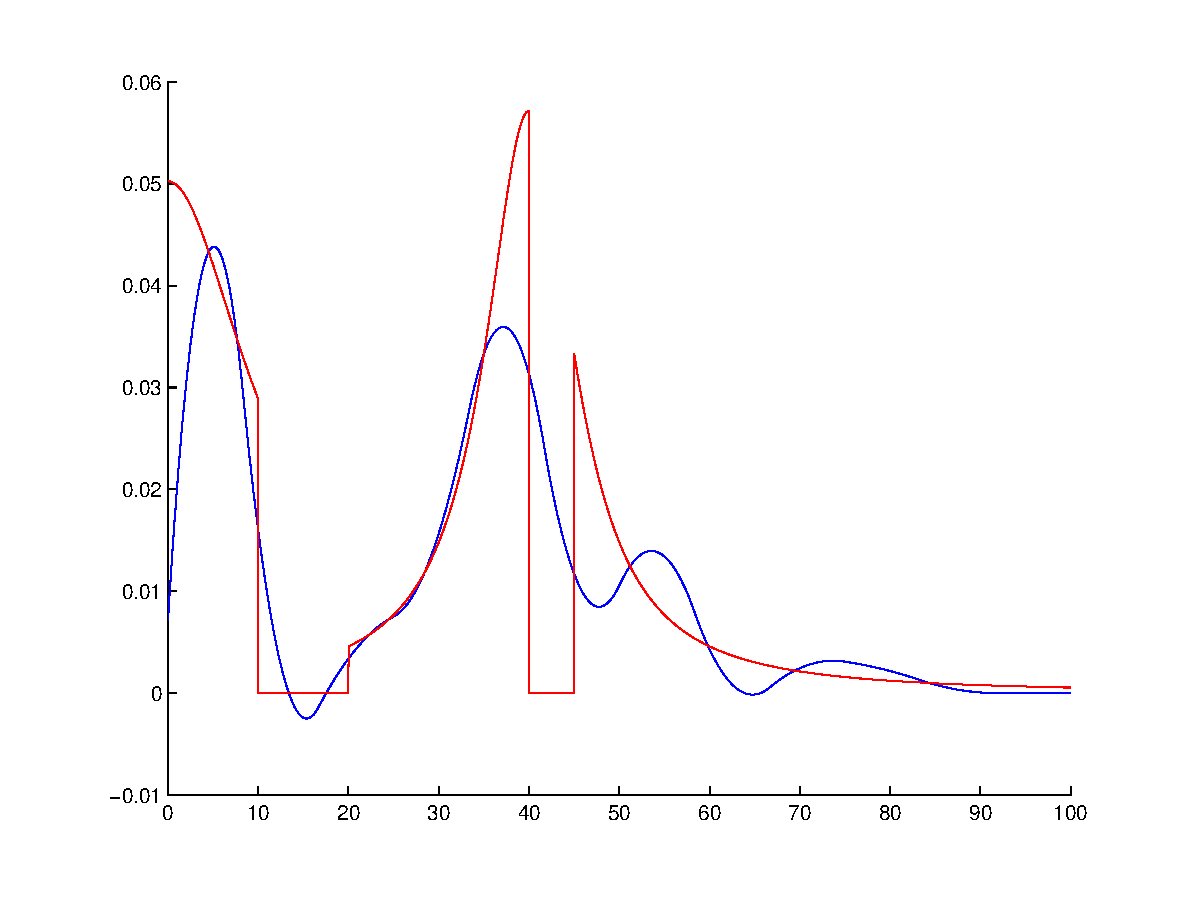
\includegraphics[scale=0.25]{pictures/Example9/Fig2.eps}
  \label{fig:9_2}
\end{minipage}%
\begin{minipage}{.33\textwidth}
  \centering
  \vspace{0.2cm}
  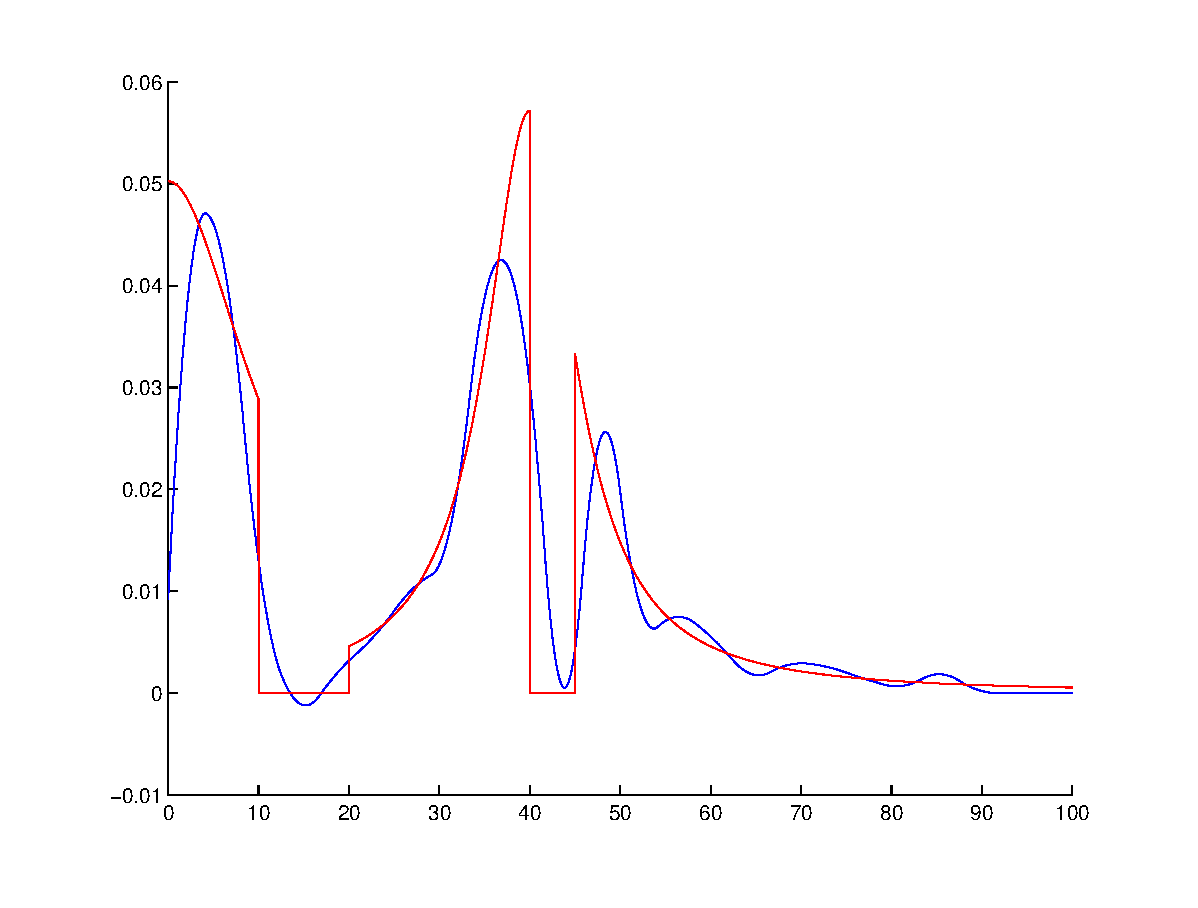
\includegraphics[scale=0.25]{pictures/Example9/Fig3.eps}
  \label{fig:9_3}
\end{minipage}%
\begin{minipage}{.33\textwidth}
  \centering
  \vspace{0.2cm}
  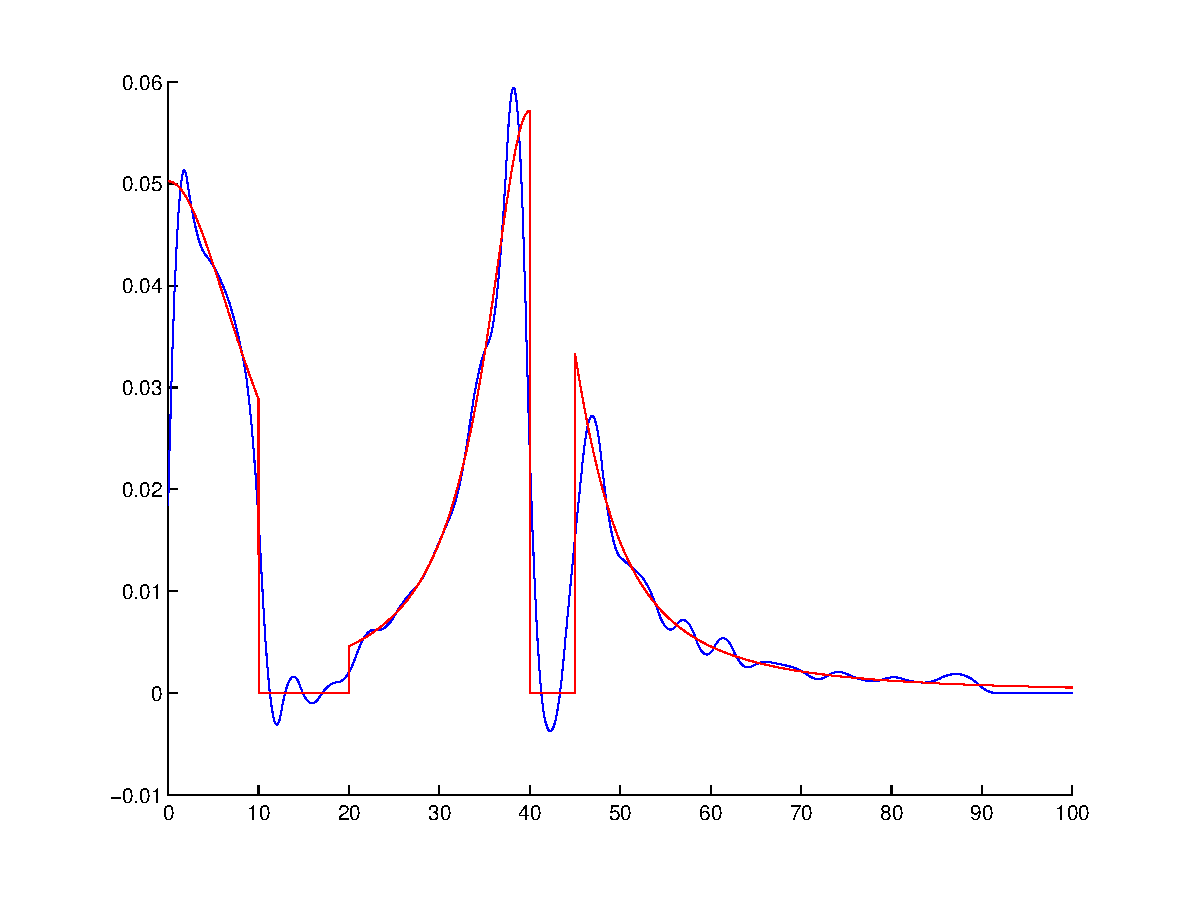
\includegraphics[scale=0.25]{pictures/Example9/Fig4.eps}
  \label{fig:9_4}
\end{minipage}%
\end{figure}

\begin{figure}[H]
\centering
\begin{minipage}{.33\textwidth}
  \centering
  \vspace{0.22cm}
  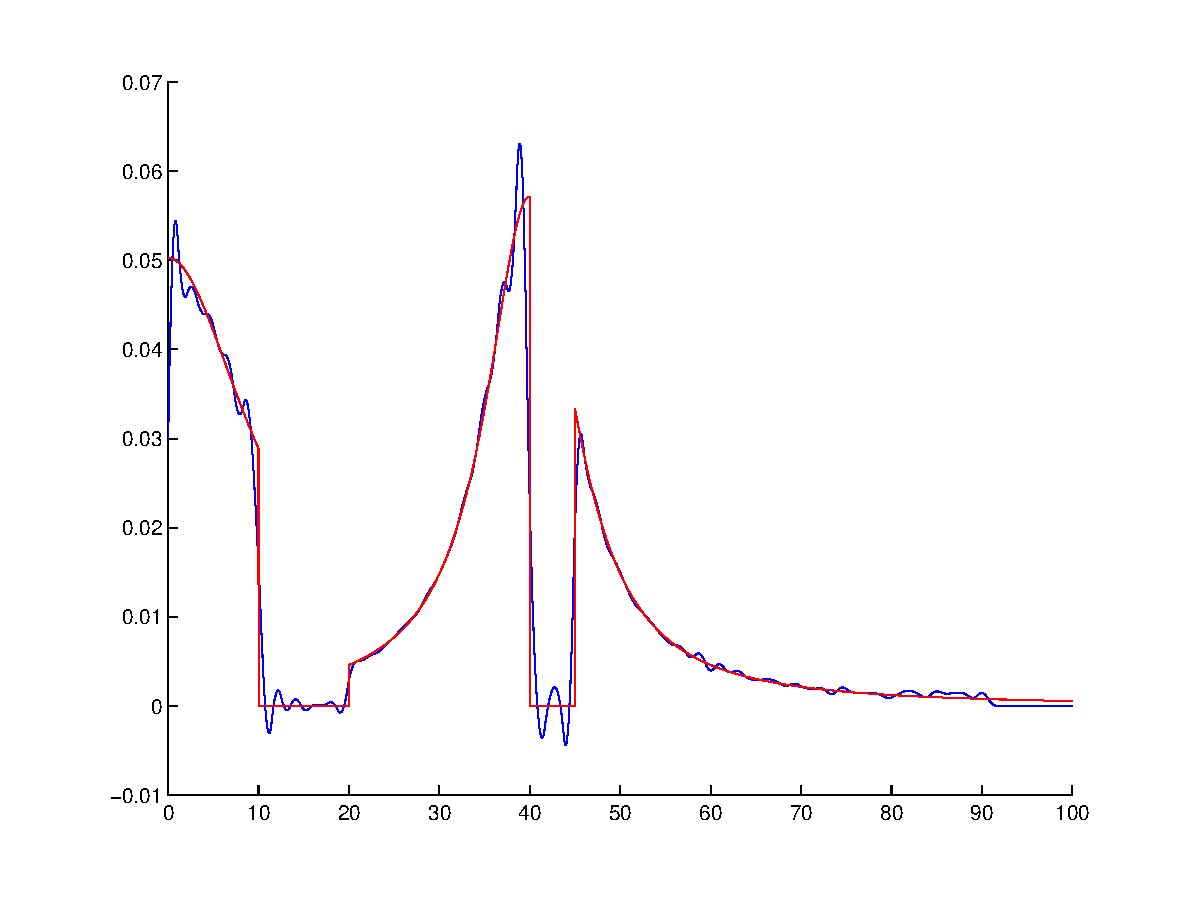
\includegraphics[scale=0.25]{pictures/Example9/Fig5.eps}
  \label{fig:9_5}
\end{minipage}%
\begin{minipage}{.33\textwidth}
  \centering
  \vspace{0.2cm}
  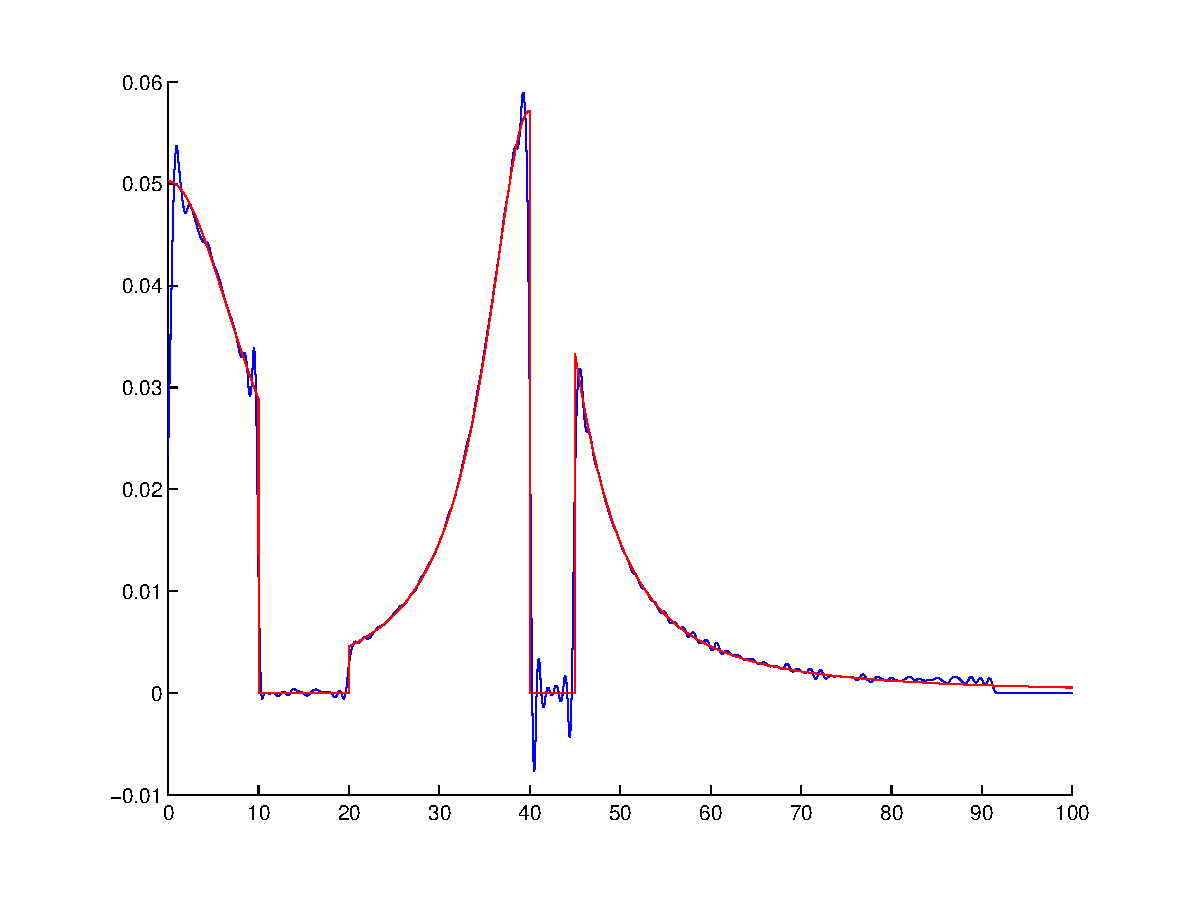
\includegraphics[scale=0.25]{pictures/Example9/Fig6.eps}
  \label{fig:9_6}
\end{minipage}%
\begin{minipage}{.33\textwidth}
  \centering
  \vspace{0.2cm}
  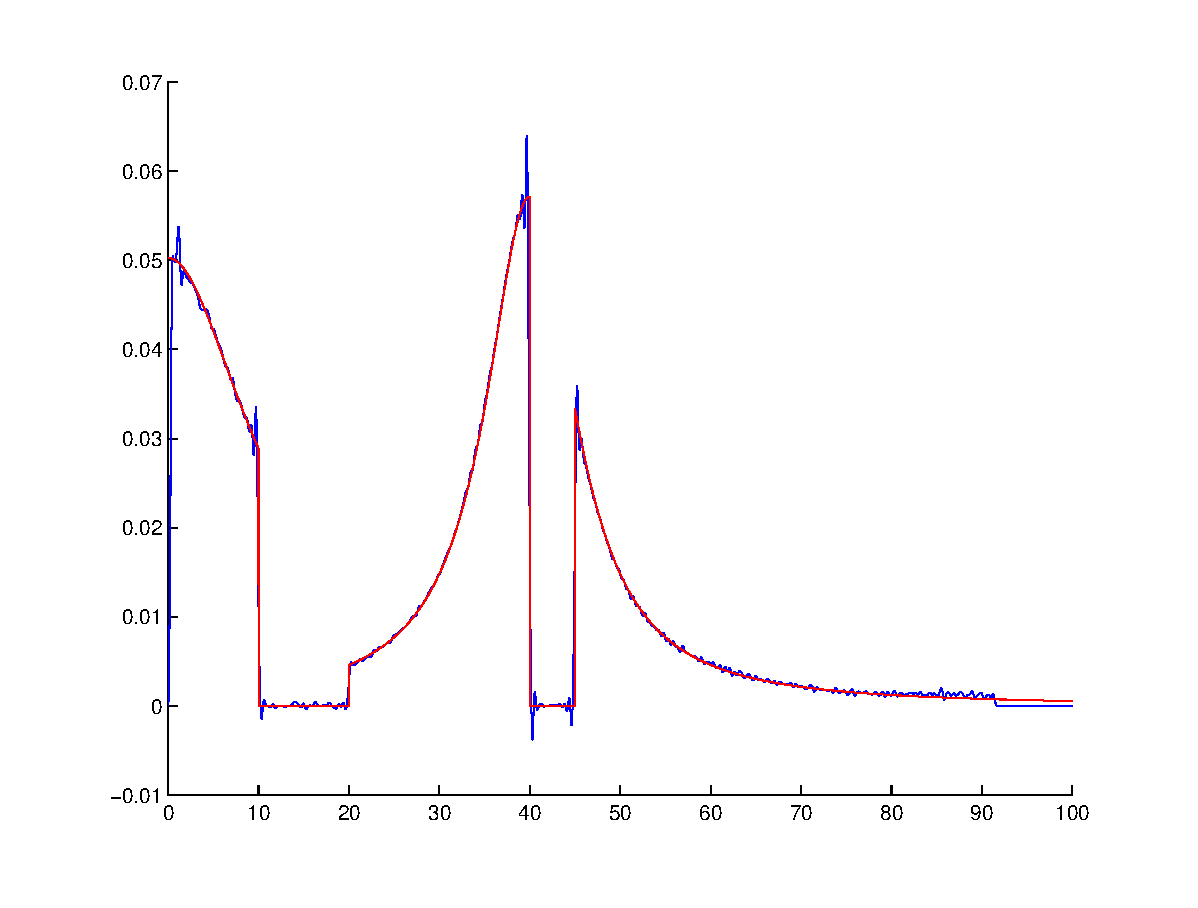
\includegraphics[scale=0.25]{pictures/Example9/Fig7.eps}
  \label{fig:9_7}
\end{minipage}%
\caption{}
\label{fig:9}
\end{figure}


\newpage

\section{Theoretical framework (as discussed with Massimo)}

Here we consider a {\bf first-order} dynamical system: More precisely, with the potential
\[
	E(x)=\sum_{i,j=1}^N A(|x_i-x_j|)
\]
the dynamical system is given by
\[
	\dot x=-\nabla E(x)\iff \dot x_i=\sum_{j=1}^N\frac{a(|x_i-x_j|)}{|x_i-x_j|}(x_j-x_i)
\]
with $N$ agents $x_j\in\R^d$, where we put $a=A'$.

We assume of the unknown function $a$ that it can be represented in some multiscale basis, i.e. that we can write
\[
	a_(r)\equiv a_\Lambda(r)\sum_{\lambda\in\Lambda}a_\lambda\varphi_\lambda\,,
\]
where $\varphi_\lambda$ are e.g. wavelet or spline functions.

First idea: Given the set $\Lambda$, we put $J_\Lambda=\bigcup_{\lambda\in\Lambda}\supp\varphi_\lambda$, and choose an interval $I_\Lambda=[t,t+\Delta t]$ such that
\[
	|x_i(s)-x_j(s)|\in J_\Lambda\qquad\forall i,j\ \forall s\in I_\Lambda\,.
\]
Then we define the functional
\begin{align*}
	\Delta^L(a,\widehat a_\Lambda)
		&=\int_t^{t+\Delta t}
			\Biggl|\biggl(\dot x_i(s)-\sum_{j=1}^N\frac{\widehat a_\Lambda(|x_i(s)-x_j(s)|)}{|x_i(s)-x_j(s)|}
				\bigl(x_j(s)-x_i(s)\bigr)\biggr)_{i=1}^N\Biggr|^2 ds\\
		&=\int_t^{t+\Delta t}\Biggl|\biggl(\sum_{j=1}^N
			\frac{a_\Lambda(|x_i(s)-x_j(s)|)-\widehat a_\Lambda(|x_i(s)-x_j(s)|)}{|x_i(s)-x_j(s)|}
			\bigl(x_j(s)-x_i(s)\bigr)\biggr)_{i=1}^N\Biggr|^2 ds\,.
\end{align*}
Of course these two versions only coincide if the $\dot x_i$ are known exactly (which generally is not true). This functional is to be optimized to find the approximation $\widehat a_\Lambda$. To ensure convergence to the true function $a_\lambda$ we need to relate $\Delta^L(a,\widehat a_\Lambda)$ to some (quasi-)norm $\|a_\Lambda-\widehat a_\Lambda\|$.

Different objective: While in this way a (good) approximation of $a_\Lambda$ may be obtained, it is equally desirable that the dynamics generated in the above way by the approximation stays close to the one generated by $a_\Lambda$.

\subsection{Upper bound}

Since for $p\leq q$ it holds $\|\alpha\|_{\ell_p}\leq N^{1/p-1/q}\|\alpha\|_{\ell_q}$, we obtain using triangle inequality
\begin{align*}
	\Delta^L(a,\widehat a_\Lambda)
		&=\int_t^{t+\Delta t}\Biggl|\biggl(\sum_{j=1}^N
			\frac{a_\Lambda(|x_i(s)-x_j(s)|)-\widehat a_\Lambda(|x_i(s)-x_j(s)|)}{|x_i(s)-x_j(s)|}
			\bigl(x_j(s)-x_i(s)\bigr)\biggr)_{i=1}^N\Biggr|_{\ell_2^N}^2 ds\\
		&=\int_t^{t+\Delta t}\sum_{i=1}^N\Bigl|\sum_{j=1}^N
			\frac{a_\Lambda(|x_i(s)-x_j(s)|)-\widehat a_\Lambda(|x_i(s)-x_j(s)|)}{|x_i(s)-x_j(s)|}
			\bigl(x_j(s)-x_i(s)\bigr)\Bigr|_{\ell_2^d}^2 ds\\
		&\leq\int_t^{t+\Delta t}\sum_{i=1}^N\Bigl(\sum_{j=1}^N
			\bigl|a_\Lambda(|x_i(s)-x_j(s)|)-\widehat a_\Lambda(|x_i(s)-x_j(s)|)\bigr|\Bigr)^2 ds\\
		&\leq N^{1/2}\int_t^{t+\Delta t}\sum_{i=1}^N\sum_{j=1}^N
			\bigl|a_\Lambda(|x_i(s)-x_j(s)|)-\widehat a_\Lambda(|x_i(s)-x_j(s)|)\bigr|^2 ds\\
		&\leq N^{1/2}|\Lambda|^{1/2}\int_t^{t+\Delta t}\sum_{i=1}^N\sum_{j=1}^N\sum_{\lambda\in\Lambda}
			\bigl|a_\lambda-\widehat a_\lambda\bigr|^2\varphi^2_\lambda(|x_i(s)-x_j(s)|) ds\,.
\end{align*}
An estimate in some weighted $\ell_2$-norm is now easily obtained, if we assume the functions $\varphi_\lambda$ to be bounded.

\subsection{Lower bound}

This time we can use Jensen's inequality
\begin{align*}
	\Delta^L(a_\Lambda,\widehat a_\Lambda)
		&\geq\frac{1}{\sqrt{\Delta t}}\Biggl\|\int_t^{t+\Delta t}\biggl(\sum_{j=1}^N
			\bigl(a_\Lambda(|z_{ij}|)-\widehat a_\Lambda(|z_{ij}|)\bigr)\sgn(z_{ji})\biggr)_{i=1}^N ds\Biggr\|^2\\
		&=\frac{1}{\sqrt{\Delta t}}\Biggl\|\int_t^{t+\Delta t}\biggl(\sum_{j=1}^N\sum_{\lambda\in\Lambda}
			(a_\lambda-\widehat a_\lambda)\varphi_\lambda(|z_{ij}|)\sgn(z_{ji})\biggr)_{i=1}^N ds\Biggr\|^2\\
		&=\frac{1}{\sqrt{\Delta t}}\Biggl\|\biggl(\int_t^{t+\Delta t}\diag\bigl(\Phi_\Lambda(s)Z(s)\bigr)ds
			(\mathbf{a}-\mathbf{\widehat a})\biggr)_{i=1}^N\Biggr\|^2\,.
\end{align*}
Here $\diag$ refers to the diagonal entries of a square matrix, in this case of $\Phi_\lambda(s)Z(s)$, which for every $\lambda\in\Lambda$ is an $N\times N$ matrix. In this way lower bounds for $\Delta^L$ can be obtained from properties of these matrices. For instance, a bound in some $\ell_2$-norm can be derived from estimates of singular values (eigenvalues) of the $|\Lambda|\times|\Lambda|$-matrix
$\diag\bigl(\Phi_\Lambda(s)Z(s)\bigr)^\top\diag\bigl(\Phi_\Lambda(s)Z(s)\bigr)$.


\subsection{Related issues}

$\bullet$ If we denote $\Gamma(a)$ the trajectories of the dynamical system generated by $a$, i.e. $\Gamma(a)(t)_i=x_i$, does $\Delta^L(a,\widehat a)$ allow assertions on the relation between $\Gamma(a)$ and $\Gamma(\widehat a)$? In other words, if $a$ is close to $\widehat a$ (in which sense?), is also $x(t)$ close to $\widehat x(t)$ (at every time $t$, or in an $L_2$-sense). Basically, we need to relate the global error on the time interval $[0,T]$ to the local error on $[t,t+\Delta t]$.

$\bullet$ If, as indicated above, $\Delta^L(a,\widehat a)$ is equivalent to $\|a-\widehat a\|_{\ell_2(\Lambda)}$, then minimizing $\Delta^L$ also gives a quasi-optimal approximation of $a$. Then, depending on the choice of the (multiscale) basis/system (wavelet, Finite element, spline), regularity of $a$ immediately transfers to convergence rates of the adaptive algorithm. Vice versa, choosing a spline basis, we can describe Besov spaces via $\Delta^L$ (since Approximation spaces for spline approximation exactly coincide with Besov spaces, as shown by DeVore and Popov, 1988)

\end{document}